% Koma-Skript Vorlage f�r Artikel
\documentclass[
    pdftex,
    a4paper,
    oneside,
    halfparskip,
    headsepline,
    footsepline,
    12pt
]{scrartcl}

% Beginn der Pr�ambel

% Paket f�r die Indexerstellung.
\usepackage{makeidx}
\makeindex 

% Paket f�r �bersetzungen ins Deutsche
% Paket f�r Rechtschreibung und Quotes
\usepackage[english]{babel}
\usepackage[babel=true]{csquotes}
% \usepackage[babel,german=swiss]{csquotes}
% \usepackage[babel,german=quotes]{csquotes} % Deutsche
% \usepackage[babel,german=swiss]{csquotes} % Schweizer
% \usepackage[babel,german=guillemets]{csquotes} % Franz�sische

% Pakete f�r Latin1 Zeichnens�tze.
% UNIX:
%\usepackage[latin1]{inputenc}
% Windows:
\usepackage[ansinew]{inputenc}

% Paket f�r TS1 Zeichens�tze
\usepackage[T1]{fontenc}

% Paket mit weiteren Symbolen
\usepackage{textcomp}

% Paket zum Erweitern der Tabelleneigenschaften
\usepackage{array}

% Paket f�r Grafiken
% \usepackage{graphicx}
\usepackage[pdftex]{graphicx}
% \usepackage{epstopdf}
% Pfad f�r Bilder, hier: alle Bilder im Unterverzeichnis Bilder
\graphicspath{{./Pictures/}}

% Paket f�r Mathematische Symbole
\usepackage{amsmath}
\usepackage{amssymb}

% Pakete f�r Type 1 Fonts (bessere Darstellung in PDF)
%\usepackage{mathptmx}             % Times + passende Mathematik-Fonts
%\usepackage[scaled=.92]{helvet}   % skalierte Helvetica als \sfdefault
\usepackage{courier}               % Courier als \ttdefault

% Paket f�r Drehungen von Elementen
\usepackage{rotating}

% Package f�r Farben
\usepackage{color}

% Paket f�r Links innerhalb des PDF Dokuments
\definecolor{LinkColor}{rgb}{0,0,0.5}
\usepackage[%
    pdftitle={Titel},%
  ]{hyperref}
\hypersetup{colorlinks=true,%
    linkcolor=LinkColor,%
    citecolor=LinkColor,%
    filecolor=LinkColor,%
    menucolor=LinkColor,%
    pagecolor=LinkColor,%
    urlcolor=LinkColor}

% Paket f�r Listings
\usepackage[savemem]{listings}
\lstloadlanguages{TeX}

\definecolor{lbcolor}{rgb}{0.85,0.85,0.85}

\lstset{language=[LaTeX]TeX,
    numbers=left,
    stepnumber=1,
    numbersep=5pt,
    numberstyle=\tiny,
    breaklines=true,
    breakautoindent=true,
    postbreak=\space,
    tabsize=2,
    basicstyle=\ttfamily\footnotesize,
    showspaces=false,
    showstringspaces=false,
    extendedchars=true,
    backgroundcolor=\color{lbcolor}}

% Index erzeugen
\makeindex

 % Allows Author-Year Bibliographies, added as a section
\usepackage{natbib}

% Setzen von Z�hlern
\setcounter{secnumdepth}{7}
\setcounter{tocdepth}{7}

% Festlegen von Kopf- und Fusszeilen
\usepackage{scrpage2}
\pagestyle{scrheadings}

% Kopfzeile:
% \ihead{innen}
% \chead{Mitte}
% \ohead{au�en}

% Fu�zeile:
% \ifoot{innen},
% \cfoot{Mitte},
% \ofoot{au�en}

\ohead{\bfseries\thepage}
   % Seitenzahl fett an den �u�eren Rand der Kopfzeile.
\automark[section]{chapter}
   % Kapiteltitel bei ungeraden Seiten (standardgem�� mittig) in die Kopfzeile.

% Paket f�r die Darstellung von "Text, wie er eingegeben wird"
% \begin{verbatim} \end{document}\end{verbatim} erzeugt die Ausgabe von
% \end{document} im Typewrites-Style und beendet nicht das Dokument.
\usepackage{verbatim}

% Paket f�r phonetische Zeichen
\usepackage{tipa}

% Paket f�r Boxen
\usepackage{fancybox}

% Ende der Pr�ambel

% Beginn des Dokumentes
\begin{document}

% Einige un�bliche Trennungen
\hyphenation
{Ur-instinkt }

% Definieren des Titels
\title{Titel}
\author{Fabian Imkenberg, Jacqueline N�ther}
\date{\today}

% Einf�gen des Titels
\maketitle

%Abstract wird voerst nicht ben�tigt
%\begin{abstract}
%In diesem Dokument werden ... vorgestellt.
%\end{abstract}

 % Umbenennen von �berschriften von Verzeichnissen
\renewcommand{\contentsname}{Content}
% Einf�gen von Verzeichnissen
\tableofcontents

% Abbildungsverzeichnis
% Einf�gen eines Seitenumbruchs
\newpage
\listoffigures

% Tabellenverzeichnis
\newpage
\listoftables

\newpage
% Einf�gen eines Abschnittes
\section{Introduction}
\label{sec:Introduction}

Dieses LaTeX Dokument stellt ... \cite{image-to-image-ccan}
\\

\begin{figure}[h]
\centering
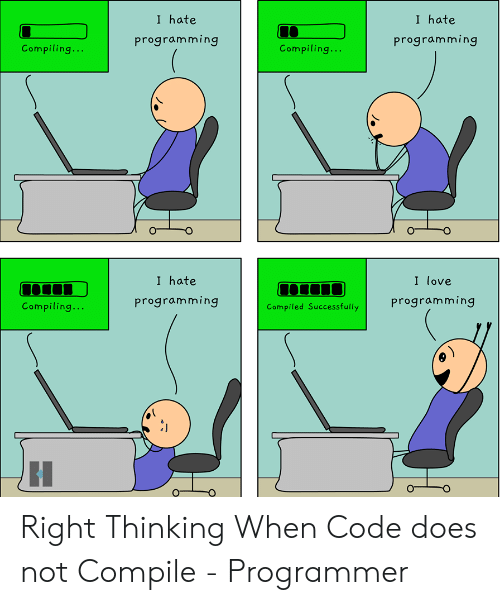
\includegraphics[scale=0.5]{test.png}
\caption{Bliblablub, dies ist eine Test-Caption}
\end{figure}
% \input{./xxx}
\section{Conclusion}
\label{sec:Conclusion}

To conclude  ... \cite{CitekeyArticle}
\\

\begin{figure}[h]
\centering
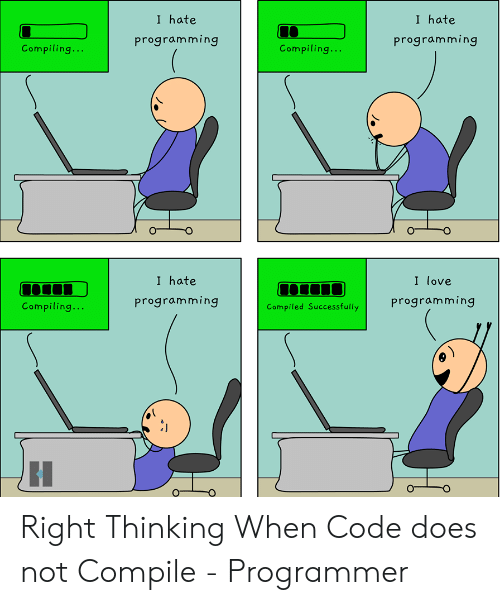
\includegraphics[scale=0.5]{test.png}
\caption{Bliblablub, dies ist eine Test-Caption}
\end{figure}



% Ab hier werden alle Abschnitte als Anh�nge betrachtet.
\appendix

% \newpage
% \section{Liste der Symbole}
% \label{sec:ListeDerSymbole}

% Anhang mit Symbolen

\newpage
% Definieren der Bibliographie
\bibliographystyle{plain}

% Externe .bib Datei
\bibliography{./references}

% Alternativ: Inline
%\begin{thebibliography}{999}
%\bibitem{homer:odyssee} Homer: Die Odyssee
%\end{thebibliography}

% Einf�gen der Bibliographie
\newpage
\addcontentsline{toc}{section}{References}

\newpage
\renewcommand{\indexname}{Abbreviations}
\addcontentsline{toc}{section}{Abbreviations}
\printindex

% Ende des Dokumentes
\end{document}
